\section[]{Templates}
   	 
   	  \subsection[]{Enumerate Auto Advance \& Alert}
   	  \begin{frame}
   	  	\frametitle{Enumerate Auto Advance \& Alert}
   	  	
   	  	\begin{enumerate}[<+- | alert@+>]
   	  		\item Textbook height in centimeters?
   	  		\item Textbook width in milimeters?
% * <nikotheteacher@gmail.com> 2016-11-26T16:21:20.335Z:
%
% ^.
% * <nikotheteacher@gmail.com> 2016-11-26T16:21:18.099Z:
%
% ^.
% * <nikotheteacher@gmail.com> 2016-11-26T16:20:28.190Z:
%
% ^.
% * <nikotheteacher@gmail.com> 2016-11-26T16:20:26.351Z:
%
% ^.
   	  		\item Notebook width in meters?
   	  		\item Whiteboard width in milimeters?
   	  	\end{enumerate}
   	  \end{frame}
   	  
   	 \subsection[]{Align Env. with Highlighting}
   	   \begin{frame}
   	   	\setcounter{equation}{0}
   	   	\begin{align}
   	   	\uncover<1->{\alert<1>{y} &= \alert<1>{mx + b} \\}
   	   	\uncover<2->{\alert<2>{m} &= \alert<2>{\dfrac{y_1 - y_2}{x_1 - x_2}}\\}
   	   	\uncover<3->{\alert<3>{m(x_1 - x_2)}&= \alert<3>{(y_1 - y_2)}\\}
   	   	\uncover<4->{\alert<4>{(y_1 - y_2)} &=  \alert<4>{m(x_1 - x_2)}\\}
   	   	\uncover<5->{\alert<5>{(y - y_2)} &=  \alert<5>{m(y - x_2)}\\}
   	   	\uncover<6->{\alert<6>{(y - y_1)} &=  \alert<6>{m(y - x_1)}}
   	   	\notag
   	   	\end{align}
   	   	\vskip-1.5em
   	   \end{frame}
   	   
   	  \subsection[]{Column Environment with equation on the left side}
   	  \begin{frame}
   	  	\frametitle{Column Environment with equation on the left side}
   	  	Some question.
   	  	
   	  	\begin{columns}
   	  		\begin{column}{0.4\textwidth}
   	  			\setcounter{equation}{0}
   	  			\begin{align}
   	  			\uncover<2->{\alert<2>{c} &= \alert<2>{\pi \times d} \\}
   	  			\uncover<3->{\alert<3>{c} & \alert<3>{\approx \dfrac{22}{7} \times 35 in}\\}
   	  			\uncover<4->{\alert<4>{c} & \alert<4>{\approx \dfrac{22}{\cancelto{1}{7}} \times \cancelto{5}{35} in}\\}
   	  			\uncover<5->{\alert<5>{c}& \alert<5>{\approx 110 in}\\}
   	  			\notag
   	  			\end{align}    	 	
   	  		\end{column}
   	  		\begin{column}{0.7\textwidth}    	
   	  		
   	  		\end{column}
   	  	\end{columns}
   	  	
   	  \end{frame}
   	  \subsection[]{Number Line I}
   	   \begin{frame}[label=PA2_01]
   	   	\frametitle{Number Line}
   	   	\NumberLine*[
   	   	dot=blue,
   	   	dot opacity=.75,
   	   	fill=blue,
   	   	fraction=1,
   	   	ticks above=false,
   	   	min=0,
   	   	number to=none,
   	   	h scale=3,
   	   	mark at={14/6,0.7,0.9},
   	   	]
   	   	\\
   	     \end{frame}   
   	     
   	   \subsection[]{Number Line II}
   	    \begin{frame}
   	      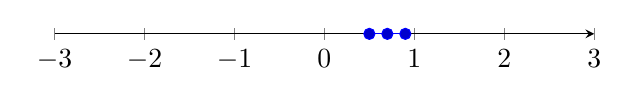
\begin{tikzpicture}
   	      \begin{axis}[
   	      axis x line=middle,
   	      % we don't need a y axis line ...
   	      axis y line=none,
   	      % ... and thus there is no need for much `height' of the axis
   	      height=50pt,
   	      % but `height' also changes `width' which is restored here
   	      width=\axisdefaultwidth,
   	      xmin=-3,
   	      xmax=3,
   	      ]
   	      \addplot coordinates {
   	      	(0.5,0) (0.7,0) (0.9,0)
   	      };
   	      \end{axis}
   	      \end{tikzpicture}   
   	     \end{frame}  	   
   	   
   	   \subsection[]{Fill in the blanks}
   	   \begin{frame}
   	   	 \frametitle{Fill in the blanks}
   	   	 \vspace*{-10pt}
   	   	\only<2>{\fillbhideanswerfalse}
   	   	\setcounter{equation}{0} 
   	   	\begin{columns}[t]
   	   		\begin{column}{0.5\textwidth}
   	   			\begin{align}
   	   			\dfrac{5}{6}\times\dfrac{\fillb{6}}{\fillb{5}} &= 1 \\
   	   			\dfrac{5}{6}\times\dfrac{\fillb{6}}{\fillb{5}} &= 1 \\
   	   			\dfrac{5}{6}\times\dfrac{\fillb{6}}{\fillb{5}} &= 1 \\
   	   			\dfrac{5}{6}\times\dfrac{\fillb{6}}{\fillb{5}} &= 1 \\
   	   			\dfrac{5}{6}\times\dfrac{\fillb{6}}{\fillb{5}} &= 1
   	   			\end{align}
   	   		\end{column}
   	   		\begin{column}{0.5\textwidth}
   	   			\begin{align}
   	   			\dfrac{5}{6}\times\dfrac{\fillb{6}}{\fillb{5}} &= 1 \\
   	   			\dfrac{5}{6}\times\dfrac{\fillb{6}}{\fillb{5}} &= 1 \\
   	   			\dfrac{5}{6}\times\dfrac{\fillb{6}}{\fillb{5}} &= 1 \\
   	   			\dfrac{5}{6}\times\dfrac{\fillb{6}}{\fillb{5}} &= 1 \\
   	   			\dfrac{5}{6}\times\dfrac{\fillb{6}}{\fillb{5}} &= 1
   	   			\end{align}
   	   		\end{column}
   	   	\end{columns}
   	   \end{frame}
   	   
   	     \subsection[]{Probability Spinner}
   	     \frametitle{Probability Spinner}
   	     \begin{frame}
   	     	\begin{tikzpicture}
   	     	\pie [sum=10, explode=0.1, text=inside,color={blue!70, green!80, red, yellow},
   	     	before number=\phantom,after number=]
   	     	{1/A, 2/, 3/Number, 4/Labels are optional}
   	     	\node [scale=3, rotate=75](note) at (0,0) {\Huge $\twoheadrightarrow$};
   	     	\end{tikzpicture}
   	     	
   	     \end{frame}	
   	   
   	   \subsection[]{Pie Chart}
   	     \frametitle{Pie Chart}
   	   \begin{frame}
   	   	 \begin{tikzpicture}
             	  \pie[sum = 10, text = legend,  explode = 0.05]{3/A , 2/B, 2/C, 3/D}
   	   	 \end{tikzpicture}
   	  
   	   \end{frame}
   	   
   	   \subsection[]{Bar Graph}
   	    \begin{frame}
   	    	\frametitle{Bar Graph}
   	    	    	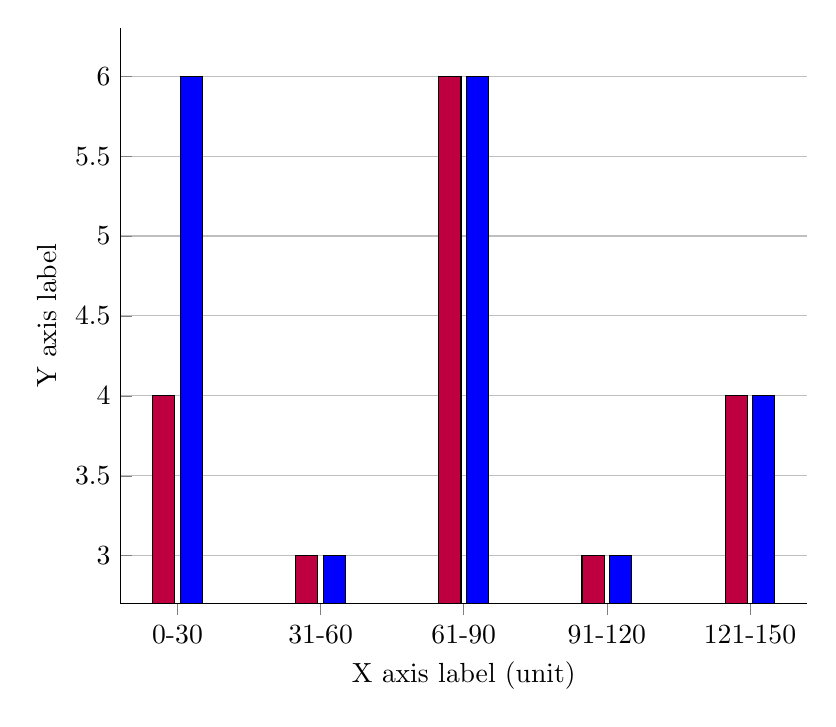
\begin{tikzpicture}
   	    	    	\begin{axis}
   	    	    	[
   	    	    	symbolic x coords={0-30, 31-60, 61-90,  91-120,  121-150, },
   	    	    	xtick=data,
   	    	    	axis lines* = left,
   	    	    	ymajorgrids= true,
   	    	    %	enlarge x limits=0.02,
   	    	        ybar,
   	    	 %       ybar interval=0.5,
   	    	        xmajorgrids= false,
   	    	        bar width=8pt, 
   	    	        width=0.85\textwidth,
   	    	    	ylabel= Y axis label, 
   	    	    	xlabel= \bluebf{X axis label (unit)}
   	    	    	]
   	    	    	\addplot[fill=purple] coordinates {
   	    	    		(0-30,  4)
   	    	    		(31-60,  3)
   	    	    		(61-90,   6)
   	    	    		(91-120,   3)
   	    	    		(121-150,   4)
   	    	    	};
   	    	    		\addplot[fill=blue] coordinates {
   	    	    			(0-30,  6)
   	    	    			(31-60,  3)
   	    	    			(61-90,   6)
   	    	    			(91-120,   3)
   	    	    			(121-150,   4)
   	    	    		};
   	    	    	\end{axis}
   	    	    	\end{tikzpicture}
   	    \end{frame}
   	    
   	    \subsection[]{Function Graph}
   	    \begin{frame}
   	    	\frametitle{Funtion Graph}
   	    	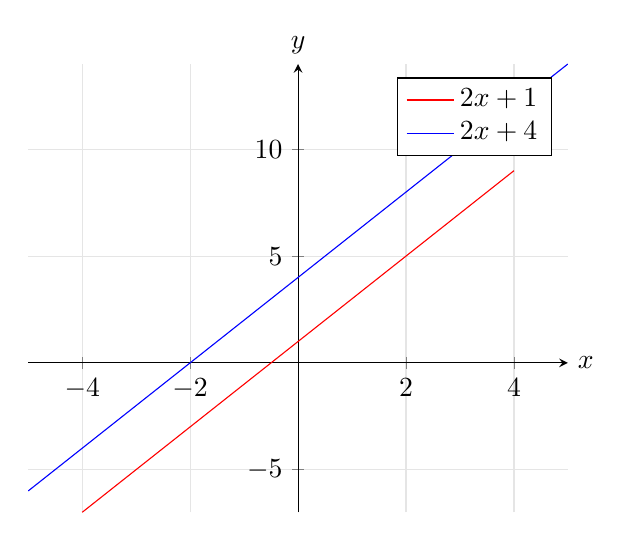
\begin{tikzpicture}
   	    	\begin{axis}[
   	    	axis lines = center,
   	    	xlabel = $x$,
   	    	xlabel style={at=(current axis.right of origin), anchor=west},
   	    	ylabel = {$y$},
   	    	ylabel style={at=(current axis.above origin), anchor=south},
   	    	%legend style = { at = {(1.0,1.0)}},
   	    	%  xtick={-5,-4,-3,-2,-1,0,1,2,3,4,5,},
   	    	% ytick={-5,-4,-3,-2,0,1,2,3,4,5},
   	    	%	enlarge y limits={rel=0.07}, 
   	    	%enlarge x limits={rel=0.07}, 
   	    	legend pos=north east,
   	    	ymajorgrids=true,
   	    	xmajorgrids=true,
   	    	grid style=  gray!20,
   	    	]
   	    	%Below the red parabola is defined
   	    	\addplot [
   	    	domain=-4:4, 
   	    	samples=100, 
   	    	color=red,
   	    	]
   	    	{2*x + 1};
   	    	\addlegendentry{$2x + 1$}
   	    	\addplot [
   	    	domain=-5:5, 
   	    	samples=100, 
   	    	color=blue,
   	    	]
   	    	{2*x + 4};
   	    	\addlegendentry{$2x + 4$}
   	    	\end{axis}
   	    	\end{tikzpicture}
   	    \end{frame}
   	    
   	    
   	    
   	    \subsection[]{Multicolored Grid}
   	    \begin{frame}
   	    	\frametitle{Fractions and Ratio}   	     	
   	    	
   	    	\begin{columns}
   	    		\begin{column}{0.5\textwidth}
   	    			What is the fraction of green squares?
   	    			\\
   	    			\smallskip
   	    			\uncover<2->{$\dfrac{3}{16}$}
   	    			\\
   	    			\bigskip
   	    			What is the ratio of red, blue and green squares?
   	    			\\
   	    			\smallskip
   	    			\uncover<3->{4:9:3}
   	    			
   	    		\end{column}
   	    		\begin{column}{0.5\textwidth}
   	    			
   	    			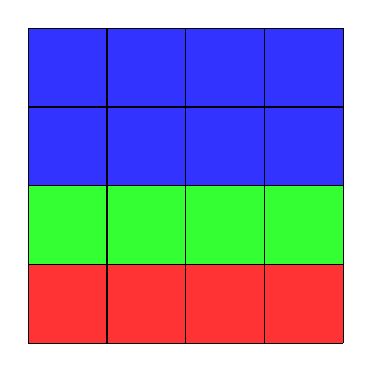
\begin{tikzpicture}[every node/.style={minimum size=1cm-\pgflinewidth, outer sep=3pt}]
   	    			\draw[step=1cm,color=black] (-1,-1) grid (3,3);
   	    			\node[fill=red!80] at (-0.5,-0.5) {};
   	    			\node[fill=red!80] at (0.5,-0.5) {};
   	    			\node[fill=red!80] at (1.5,-0.5) {};
   	    			\node[fill=red!80] at (2.5,-0.5) {};
   	    			\node[fill=green!80] at (-0.5,0.5) {};
   	    			\node[fill=green!80] at (0.5,0.5) {};
   	    			\node[fill=green!80] at (1.5,0.5) {};
   	    			\node[fill=green!80] at (2.5,0.5) {};
   	    			\node[fill=blue!80] at (-0.5,1.5) {};
   	    			\node[fill=blue!80] at (0.5,1.5) {};
   	    			\node[fill=blue!80] at (1.5,1.5) {};
   	    			\node[fill=blue!80] at (2.5,1.5) {};
   	    			\node[fill=blue!80] at (-0.5,2.5) {};
   	    			\node[fill=blue!80] at (0.5,2.5) {};
   	    			\node[fill=blue!80] at (1.5,2.5) {};
   	    			\node[fill=blue!80] at (2.5,2.5) {};
   	    			\end{tikzpicture}
   	    			
   	    		\end{column}
   	    		
   	    	\end{columns}
   	    \end{frame}
   	    
   	    \subsection[]{Co-ordinate Drawing - Labelled Star}
   	    	\begin{frame}
   	    		\frametitle{Co-ordinate Drawing}
   	    		
   	    		\begin{center}
   	    			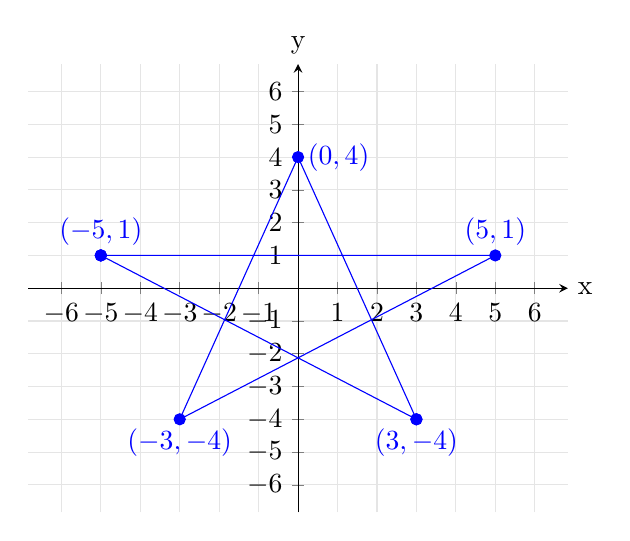
\begin{tikzpicture}
   	    			\begin{axis}[
   	    			axis lines = center, %left, center, right
   	    			%	title={Stone in Free-fall},
   	    			xlabel={x},
   	    			xlabel style={at=(current axis.right of origin), anchor=west},
   	    			ylabel={y},
   	    			ylabel style={at=(current axis.above origin), anchor=south},
   	    			xmin=-6, xmax=6,
   	    			ymin=-6, ymax=6,
   	    			xtick={-6,-5,-4,-3,-2,-1,0,1,2,3,4,5,6},
   	    			ytick={-6,-5,-4,-3,-2,-1,0,1,2,3,4,5,6},
   	    			enlarge y limits={rel=0.07}, 
   	    			enlarge x limits={rel=0.07}, 
   	    			legend pos=north east,
   	    			ymajorgrids=true,
   	    			xmajorgrids=true,
   	    			grid style=  gray!20,
   	    			]
   	    			
   	    			\addplot [
   	    			color=blue,
   	    			mark=*, % * is a filled circle, other options are square
   	    			%only marks,
   	    			]
   	    			coordinates {
   	    				(-5,1)(3,-4)(-5,1)(5,1)(-3,-4)(0,4)(3,-4)(-5,1)
   	    			}
   	    			%     \node[anchor=north] at (axis cs:2,1) {$f(\theta_A, x)$};
   	    			%	  node[pin={$(2,-1)$}] at (axis cs: 2,1) {}
   	    			node [anchor=south] at (axis cs: -5,1) {$(-5,1)$}
   	    			node [anchor=south] at (axis cs: 5,1) {$(5,1)$}
   	    			node [anchor=west] at (axis cs: 0,4) {$(0,4)$}
   	    			node [anchor=north] at (axis cs: -3,-4) {$(-3,-4)$}
   	    			node [anchor=north] at (axis cs: 3,-4) {$(3,-4)$}
   	    			;
   	    			
   	    			\end{axis}
   	    			\end{tikzpicture} 
   	    		\end{center}
   	    		
   	    	\end{frame}
   	    
   	     \subsection[]{Triangle}
   	     \begin{frame}
   	     	\frametitle{Triangle}
   	        \begin{tikzpicture}[thick,color=crimson]
   	        \coordinate (O) at (0,0);
   	        \coordinate (A) at (4,0);
   	        \coordinate (B) at (2.4,2.2);
   	        \draw (O)--(A)--(B)--cycle;
   	        
   	        \tkzLabelSegment[below=2pt](O,A){$2(x + 4)$ cm}
   	        \tkzLabelSegment[left=6pt](O,B){$3x$ cm}
   	        \tkzLabelSegment[above right=2pt](A,B){$2x + 1$ cm}
   	        \end{tikzpicture} 
   	     \end{frame}
   	     \subsubsection{Isosceles Triangle}
   	     \begin{frame}
   	     	\frametitle{Isosceles Triangle}
   	     	
   	     	\begin{tikzpicture}[scale=1]
   	     	\tkzDefPoints{0/0/O,2/2/A,4/0/B,6/2/C}
   	     	\tkzDrawSegments(O,A A,B)
   	     	\tkzDrawPoints(O,A,B)
   	     	\tkzDrawLine(O,B)
   	     	\tkzMarkSegments[mark=|,size=4pt](O,A A,B)
   	     	\end{tikzpicture}
   	     	
   	     \end{frame}
   	     
   	     \subsection[]{Rectangle}
   	         \begin{frame}
   	         	\frametitle{Rectangle}
   	         	\begin{tikzpicture}[thick,color=crimson]
   	         	\coordinate (O) at (0,0);
   	         	\coordinate (A) at (4,0);
   	         	\coordinate (B) at (4,4);
   	         	\coordinate (C) at (0,4);
   	         	\draw (O)--(A)--(B)--(C)--cycle;
   	         	
   	         	\tkzLabelSegment[below=2pt](O,A){$2(x + 4)$ cm}
   	         	\tkzLabelSegment[left=6pt](O,B){$3x$ cm}
   	         	\tkzLabelSegment[above right=2pt](A,B){$2x + 1$ cm}
   	         	\end{tikzpicture} 
   	         \end{frame}
   	         
   	         \subsection[]{Circle}
   	           \begin{frame}
   	           	  \frametitle{Circle Ring}
   	            \begin{tikzpicture}[scale=2]
   	            \tkzDefPoint(0,0){O}
   	            \tkzDefPoint(1,0){A}
   	             \tkzDefPoint(-1.5,0){B}
   	             \tkzDefPoint(-1.6,0){r_1=3}
   	              \tkzDefPoint(0,1){C}
   	               \tkzDefPoint(0,0.6){r_2=2}
   	             \tkzDrawCircle[color=blue, fill = blue](O,B)
   	            \tkzDrawCircle[color=red, fill = red](O,A)
   	            \tkzDrawSegments[color=black,ultra thick](C,O O,B)
   	            \tkzLabelPoints[color=green, ultra thick](r_1=3)
   	              \tkzLabelPoints[color=green, ultra thick](r_2=2)
   	           
   	            \end{tikzpicture} 
   	             \end{frame}
   	             
   	             \begin{frame}
   	             	\frametitle{Semi Circle}
   	             	\begin{tikzpicture}[scale=.75]
   	             	\tkzInit[ymax=8,xmax=8]
   	             	%	\tkzClip[space=.25]
   	             	\tkzDefPoint(0,0){A}
   	             	\tkzDefPoint(8,0){B} 
   	             	\tkzDefPoint(4,0){O}
   	             	\tkzDrawSector[fill=yellow](O,B)(A)
   	             	\tkzDrawPoints(A,B,O)
   	             	\tkzLabelPoints(A,B,O)
   	             	\tkzLabelSegment[below=2pt](A,O){$\overline{A0}=4$}
   	             	\end{tikzpicture}
   	             \end{frame}
   	         
   	            \begin{frame}
   	              \frametitle{Circle Arc I}
   	              
   	             \begin{tikzpicture}
   	             \tkzInit[ymin=-2.25,ymax=2.25,xmin=-2.25,xmax=2.25]
   	             \tkzDefPoint(0,0){O}
   	             \tkzDefPoint(2,0){N}
   	             \tkzDefPointBy[rotation=center O angle 20](N)
   	             \tkzGetPoint{M}
   	             \tkzDefPointBy[rotation=center O angle -20](N)
   	             \tkzGetPoint{P}
   	             \tkzDefPointBy[rotation=center O angle 125](N)
   	             \tkzGetPoint{P’}
   	             \tkzLabelCircle[above=4pt](O,N)(120){Label}
   	             \tkzDrawCircle(O,M)
   	             \tkzFillCircle[color=blue!20,opacity=.4](O,M)
   	             \tkzLabelCircle[R,draw,fill=orange!30,%
   	             text width=2cm,text centered](O,3 cm)(-60)%
   	             {Label}
   	             \tkzDrawSegment[dashed](O,P)
   	             \tkzDrawSegment[dashed](O,M)
   	             \tkzDrawPoints(M,P)\tkzLabelPoints[right](M,P)
   	             \end{tikzpicture}
   	             
   	            \end{frame}
   	         
   	             \begin{frame}
   	             	\frametitle{Circle Chrod and Arc}
   	             	
   	             	\begin{tikzpicture}[scale=1.5]
   	             	\tkzDefPoint(0,0){O}
   	             	\tkzDefPoint(2,0.5){A}
   	             	\tkzDefPointBy[rotation= center O angle 30](A)
   	             	\tkzGetPoint{B}
   	             	\tkzDrawArc[color=blue, thick](O,A)(B)
   	             	\tkzDrawArc(O,B)(A)
   	             	\tkzDrawLines[add = 0 and .5](O,A O,B)
   	             	\tkzLabelLine[above, rotate=48](O,B){$\overline{OB}=2m$}
   	             	\tkzDrawPoints(O,A,B)
   	             	\tkzLabelPoints[below](O,A,B)
   	             	\tkzLabelAngle[color=blue, rotate = 18](A,O,B){$\measuredangle = 30\degree$}
   	             	\tkzFillSector[rotate,color=orange!70,opacity=0.2](O,B)(330)
   	             	\tkzFillSector[rotate,color=blue!70,opacity=0.4](O,A)(30)
   	             	\end{tikzpicture}
   	             	
   	             \end{frame}
                 
 \subsection[]{Probability Trees}
   \subsubsection{Probability Tree - Two Coins}
   	\begin{frame}{Probability Tree - Two Coins}
      \begin{tikzpicture}[grow=right, sloped]
 		\tikzstyle{level 1}=[level distance=3.5cm, sibling distance=3.5cm]
		\tikzstyle{level 2}=[level distance=3.5cm, sibling distance=2cm]
		\tikzstyle{toss} = [text width=4em, text centered]
		\tikzstyle{end} = [circle, minimum width=3pt,fill, inner sep=0pt]
			\node[toss] {Coin 1}
				child<2-> {
				   node[toss] {Tails}
						child<3-> {
					    node[toss,label=right:{label}] {Head}
                              }
				       child<3-> {
	    			    node[toss] {Tails}
							}
					       }
				child<4-> {
					node[toss] {Head}
						child<5-> {
							node[toss] {Tails}
									}
						 child<6-> {
						    node[toss] {This could be an image}
								}		
						}
 					;				
		\end{tikzpicture}                 
                 \end{frame}
           
           
           \subsubsection{Probability Trees - Two Coins Downward}
           \begin{frame}{Probability Tree - Two Coins $\Downarrow$}
           	\begin{tikzpicture}[grow=down, sloped]
           	\tikzstyle{level 1}=[level distance=1.5cm, sibling distance=4cm]
           	\tikzstyle{level 2}=[level distance=1.5cm, sibling distance=2.5cm]
           	\tikzstyle{toss} = [text width=4em, text centered]
           	\tikzstyle{end} = [circle, minimum width=3pt,fill, inner sep=0pt]
           	\node[toss] {\includegraphics[width=0.4\linewidth]{Images/coin}}
           	child<2-> {
           		node[toss] {Tails}
           		child<6-> {
           			node[toss,label=below:{\bluebf{TH}}] {Head}
           		}
           		child<5-> {
           			node[toss,label=below:{\bluebf{TT}}] {Tails}
           		}
           	}
           	child<2-> {
           		node[toss] {Head}
           		child<4-> {
           			node[toss,label=below:{\redbf{HT}}] {Tails}
           		}
           		child<3-> {
           			node[toss,label=below:{\redbf{HH}}] {Head}
           		}		
           	}
           	;				
           	\end{tikzpicture}                 
           \end{frame}
           
           \subsubsection{Probability Tree - Die and Coin Downward}               
           \begin{frame}{Probability Tree - Die and Coin}
           	%	\begin{center}
           	\hspace*{-20pt}	\begin{tikzpicture}[grow=down, sloped]
           	\tikzstyle{level 1}=[level distance=1.5cm, sibling distance=1.8cm]
           	\tikzstyle{level 2}=[level distance=1.5cm, sibling distance=1cm]
           	\tikzstyle{toss} = [text width=4em, text centered]
           	\tikzstyle{end} = [circle, minimum width=3pt,fill, inner sep=0pt]
           	\node[toss] {\includegraphics[width=0.4\linewidth]{Images/dice}}
           	child<2-> {
           		node[toss] {1}
           		child<3-> {
           			node[toss,label=below:{\bluebf{1T}}] {T}
           		}
           		child<3-> {
           			node[toss,label=below:{\bluebf{1H}}] {H}
           		}
           	}
           	child<2-> {
           		node[toss] {2}
           		child<4-> {
           			node[toss,label=below:{\redbf{2T}}] {T}
           		}
           		child<4-> {
           			node[toss,label=below:{\redbf{2H}}] {H}
           		}		
           	}
           	child<2-> {
           		node[toss] {3}
           		child<5-> {
           			node[toss,label=below:{\bluebf{3T}}] {T}
           		}
           		child<5-> {
           			node[toss,label=below:{\bluebf{3H}}] {H}
           		}
           	}
           	child<2-> {
           		node[toss] {4}
           		child<5-> {
           			node[toss,label=below:{\redbf{4T}}] {T}
           		}
           		child<5-> {
           			node[toss,label=below:{\redbf{4H}}] {H}
           		}		
           	}
           	child<2-> {
           		node[toss] {5}
           		child<5-> {
           			node[toss,label=below:{\bluebf{5T}}] {T}
           		}
           		child<5-> {
           			node[toss,label=below:{\bluebf{5H}}] {H}
           		}
           	}
           	child<2-> {
           		node[toss] {6}
           		child<5-> {
           			node[toss,label=below:{\redbf{6T}}] {T}
           		}
           		child<5-> {
           			node[toss,label=below:{\redbf{6H}}] {H}
           		}		
           	}
           	;				
           	\end{tikzpicture}    
           	%	\end{center}             
           \end{frame}
           \subsubsection{Probability Tree - Coin \& Die Downward}               
           \begin{frame}{Probability Tree - Coin \& Die}
           	%	\begin{center}
           	\hspace*{-30pt}
           	\begin{tikzpicture}[grow=down, sloped]
           	\tikzstyle{level 1}=[level distance=1.2cm, sibling distance=6cm]
           	\tikzstyle{level 2}=[level distance=1.8cm, sibling distance=1cm]
           	\tikzstyle{toss} = [text width=4em, text centered]
           	\tikzstyle{end} = [circle, minimum width=3pt,fill, inner sep=0pt]
           	\node[toss] {\includegraphics[width=0.4\linewidth]{Images/coin}}
           	child<2-> {
           		node[toss] {Head}
           		child<3-> {
           			node[toss,label=below:{\bluebf{H1}}] {1}
           		}
           		child<3-> {
           			node[toss,label=below:{\bluebf{H2}}] {2}
           		}
           		child<3-> {
           			node[toss,label=below:{\bluebf{H3}}] {3}
           		}
           		child<3-> {
           			node[toss,label=below:{\bluebf{H4}}] {4}
           		}
           		child<3-> {
           			node[toss,label=below:{\bluebf{H5}}] {5}
           		}
           		child<3-> {
           			node[toss,label=below:{\bluebf{H6}}] {6}
           		}
           	}
           	child<2-> {
           		node[toss] {Tail}
           		child<4-> {
           			node[toss,label=below:{\redbf{T1}}] {1}
           		}
           		child<4-> {
           			node[toss,label=below:{\redbf{T2}}] {2}
           		}	
           		child<4-> {
           			node[toss,label=below:{\redbf{T3}}] {3}
           		}
           		child<4-> {
           			node[toss,label=below:{\redbf{T4}}] {4}
           		}
           		child<4-> {
           			node[toss,label=below:{\redbf{T5}}] {5}
           		}
           		child<4-> {
           			node[toss,label=below:{\redbf{T6}}] {6}
           		}	
           	}
           	;				
           	\end{tikzpicture}    
           	%	\end{center}             
           \end{frame}
                 
   	      	     \subsection[]{Sample Space - Pair of Dice}
   	      	     \begin{frame}
   	      	     	\frametitle{Sample Space - Pair of Dice B \& W}
   	      	     	$	\begin{array}{ccccccc}
   	      	     	& {\large \bluebf{\epsdice{1}}} & {\large \bluebf{\epsdice{2}}}  & {\large \bluebf{\epsdice{3}}}  & {\large \bluebf{\epsdice{4}}}  &  {\large \bluebf{\epsdice{5}}} &  {\large \bluebf{\epsdice{6}}} \\ 
   	      	     	{\large {\epsdice[black]{1}}}  	& 2 & 3 & 4 & 5 & 6 & 7  \\ 
   	      	     	{\large {\epsdice[black]{2}}}    & 3 & 4 & 5 & 6 & 7 & 8  \\ 
   	      	     	{\large {\epsdice[black]{3}}}    & 4 & 5 & 6 & 7 & 8 & 9  \\ 
   	      	     	{\large {\epsdice[black]{4}}}    & 5 & 6 & 7 & 8 & 9 & 10 \\ 
   	      	     	{\large {\epsdice[black]{5}}}   	& 6 & 7 & 8 & 9 & 10 & 11 \\ 
   	      	     	{\large {\epsdice[black]{6}}}   	& 7 & 8 & 9 & 10 & 11 & 12
   	      	     	\end{array} $
   	      	     \end{frame}
   	      	     
   	      	     \begin{frame}
   	      	     	\frametitle{Sample Space - Pair of Dice Blue \& Red}
   	      	     	
   	      	     	$	\begin{array}{ccccccc}
   	      	     	& \bluebf{\Cube{1}}   & \bluebf{\Cube{2}} & \bluebf{\Cube{3}}  & \bluebf{\Cube{4}}  &  \bluebf{\Cube{5}} &  \bluebf{\Cube{6}} \\ 
   	      	     	\redbf{\Cube{1}}     		& 2 & 3 & 4 & 5 & 6 & 7 \\ 
   	      	     	\redbf{\Cube{2}}       	& 3 & 4 & 5 & 6 & 7 & 8 \\ 
   	      	     	\redbf{\Cube{3}}       	& 4 & 5 & 6 & 7 & 8 & 9 \\ 
   	      	     	\redbf{\Cube{4}}      	& 5 & 6 & 7 & 8 & 9 & 10 \\ 
   	      	     	\redbf{\Cube{5}}     		& 6 & 7 & 8 & 9 & 10 & 11 \\ 
   	      	     	\redbf{\Cube{6}}   		& 7 & 8 & 9 & 10 & 11 & 12
   	      	     	\end{array} $
   	      	     	
   	      	     \end{frame}
   	      	     
   	      	       \subsection[]{Sample Space - A die and Spinner}
   	      	       
   	      	         \begin{frame}   	      	       
   	      	           \frametitle{Probability - A die and Spinner}
   	      	           
   	      	           A 6 number die is tossed and the spinner spun at the same time. What is the probability that the letter J and an odd number will turn up?
   	      	           
   	      	           \begin{columns}[b]
   	      	           	\column{0.5\textwidth}{
   	      	           		\begin{center}
   	      	           			\includegraphics[width=0.5\linewidth]{Images/dice}
   	      	           		\end{center}
   	      	           	}
   	      	           	\column{0.5\textwidth}{
   	      	           		\begin{center}
   	      	           			\begin{tikzpicture}[scale=0.5]
   	      	           			\pie [sum=5, text=inside,
   	      	           			before number=\phantom,after number=]
   	      	           			{1/J, 1/K, 1/L, 1/M,1/N}
   	      	           			\node [scale=1.4, rotate=90](note) at (0,0) {\Huge $\twoheadrightarrow$};
   	      	           			\end{tikzpicture}
   	      	           		\end{center}
   	      	           	}
   	      	           \end{columns}
   	      	        \end{frame}
   	      	        
   	      	           \begin{frame}
   	      	        	\frametitle{Question of the day - Probability}
   	      	        	A 6 number die is tossed and the spinner spun at the same time. What is the probability that the letter J and an odd number will turn up?
   	      	        	\\
   	      	        	\bigskip
   	      	        	\pause
   	      	        	First we need to determine the sample space.
   	      	        	\\
   	      	        	\bigskip
   	      	        	\pause
   	      	        	$	\begin{array}{ccccccc}
   	      	        	& \bluebf{J} & \bluebf{K}  & \bluebf{L}  &  \bluebf{M} &  \bluebf{N} \\ 
   	      	        	\redbf{\Cube{1}}     	& J1 & K1 & L1 & M1 & N1  \\ 
   	      	        	\redbf{\Cube{2}}       	& J2 & K2 & L2 & M2 & N2  \\ 
   	      	        	\redbf{\Cube{3}}       	& J3 & K3 & L3 & M3 & N3  \\ 
   	      	        	\redbf{\Cube{4}}      	& J4 & K4 & L4 & M4 & N4  \\ 
   	      	        	\redbf{\Cube{5}}     	& J5 & K5 & L5 & M5 & N5  \\ 
   	      	        	\redbf{\Cube{6}}   		& J6 & K6 & L6 & M6 & N6 
   	      	        	\end{array} $
   	      	        	
   	      	        \end{frame}
   	      	        
   	      	        	\begin{frame}
   	      	        		\frametitle{Question of the day - Probability}
   	      	        		A 6 number die is tossed and the spinner spun at the same time. What is the probability that the letter J and an odd number will turn up?
   	      	        		\\
   	      	        		\bigskip
   	      	        		What are the favorable outcomes?
   	      	        		\\
   	      	        		\bigskip
   	      	        		$	\begin{array}{ccccccc}
   	      	        		& \bluebf{J} & \bluebf{K}  & \bluebf{L}  &  \bluebf{M} &  \bluebf{N} \\ 
   	      	        		\redbf{\Cube{1}}     	& J1 & K1 & L1 & M1 & N1  \\ 
   	      	        		\redbf{\Cube{2}}       	& J2 & K2 & L2 & M2 & N2  \\ 
   	      	        		\redbf{\Cube{3}}       	& J3 & K3 & L3 & M3 & N3  \\ 
   	      	        		\redbf{\Cube{4}}      	& J4 & K4 & L4 & M4 & N4  \\ 
   	      	        		\redbf{\Cube{5}}     	& J5 & K5 & L5 & M5 & N5  \\ 
   	      	        		\redbf{\Cube{6}}   		& J6 & K6 & L6 & M6 & N6 
   	      	        		\end{array} $
   	      	        		
   	      	        	\end{frame}
   	      	        	
   	      	        	\begin{frame}
   	      	        		\frametitle{Question of the day - Probability}
   	      	        		A 6 number die is tossed and the spinner spun at the same time. What is the probability that the letter J and an odd number will turn up?
   	      	        		\\
   	      	        		\bigskip
   	      	        		What are the favorable outcomes?
   	      	        		\\
   	      	        		\bigskip
   	      	        		$	\begin{array}{ccccccc}
   	      	        		& \bluebf{J} & \bluebf{K}  & \bluebf{L}  &  \bluebf{M} &  \bluebf{N} \\ 
   	      	        		\redbf{\Cube{1}}     	& \greenbf{J1} & K1 & L1 & M1 & N1  \\ 
   	      	        		\redbf{\Cube{2}}       	& J2 & K2 & L2 & M2 & N2  \\ 
   	      	        		\redbf{\Cube{3}}       	& \greenbf{J3} & K3 & L3 & M3 & N3  \\ 
   	      	        		\redbf{\Cube{4}}      	& J4 & K4 & L4 & M4 & N4  \\ 
   	      	        		\redbf{\Cube{5}}     	& \greenbf{J5} & K5 & L5 & M5 & N5  \\ 
   	      	        		\redbf{\Cube{6}}   		& J6 & K6 & L6 & M6 & N6 
   	      	        		\end{array} $
   	      	        		
   	      	        	\end{frame}
   	      	        	
   	      	        	\begin{frame}
   	      	        		\frametitle{Question of the day - Probability}
   	      	        		A 6 number die is tossed and the spinner spun at the same time. What is the probability that the letter J and an odd number will turn up?
   	      	        		\\
   	      	        		\bigskip
   	      	        		\fbox{$Probability = \dfrac{3}{36} \Longrightarrow \dfrac{1}{12} $}
   	      	        		\\
   	      	        		\bigskip
   	      	        		$	\begin{array}{ccccccc}
   	      	        		& \bluebf{J} & \bluebf{K}  & \bluebf{L}  &  \bluebf{M} &  \bluebf{N} \\ 
   	      	        		\redbf{\Cube{1}}     	& \greenbf{J1} & K1 & L1 & M1 & N1  \\ 
   	      	        		\redbf{\Cube{2}}       	& J2 & K2 & L2 & M2 & N2  \\ 
   	      	        		\redbf{\Cube{3}}       	& \greenbf{J3} & K3 & L3 & M3 & N3  \\ 
   	      	        		\redbf{\Cube{4}}      	& J4 & K4 & L4 & M4 & N4  \\ 
   	      	        		\redbf{\Cube{5}}     	& \greenbf{J5} & K5 & L5 & M5 & N5  \\ 
   	      	        		\redbf{\Cube{6}}   		& J6 & K6 & L6 & M6 & N6 
   	      	        		\end{array} $
   	      	        		
   	      	        	\end{frame}
   	     \subsection[]{Fancy Pi}
   	     \begin{frame}
   	     	\frametitle{Fancy Pi}
   	     	
   	     	   \def\defaultstartht{20pt}
   	     	   \diminish[0.97]{\pinum}
   	     	   
   	     \end{frame}
   	     